\documentclass{article}
\usepackage{amsfonts}
\usepackage{amsthm}
\usepackage{amssymb}
\usepackage{amsmath}
\usepackage{graphicx}
\usepackage{subcaption}
\usepackage{xcolor}
\usepackage{mathtools}
\usepackage{ wasysym }
\usepackage{enumerate}
\usepackage{verbatim}


\numberwithin{equation}{section}
\newcommand{\new}[2]{
    \vspace{2mm}
    \noindent
    \textbf{
    \underline{#1}}
    \textit{{#2}}
    \
}

\def\<{{\langle}}
\def\>{{\rangle}}

\DeclarePairedDelimiter\bra{\langle}{\rvert}
\DeclarePairedDelimiter\ket{\lvert}{\rangle}
\DeclarePairedDelimiterX\braket[2]{\langle}{\rangle}{#1\,\delimsize\vert\,\mathopen{}#2}


\newcommand{\textOr}{
    {
        \hspace{5mm}
        \textrm{or}
        \hspace{5mm}
    }
}

\newcommand{\textAnd}{
    {
        \hspace{5mm}
        \textrm{and}
        \hspace{5mm}
    }
}


\newcommand{\textWhere}{
    {
        \hspace{5mm}
        \textrm{where}
        \hspace{5mm}
    }
}



\newcommand{\Ixp}[1]{
    {
        e^{i{#1}}
    }
}



\newcommand{\halfFigure}[1]{
\begin{center}
\includegraphics[width = .5\linewidth]{{#1}}
\end{center}
}

\newcommand{\fullFigure}[1]{
\begin{center}
\includegraphics[width = .9\linewidth]{{#1}}
\end{center}
}

\def\twobytwoMat(#1, #2, #3, #4){
    {
        \begin{bmatrix}
            {#1} & {#2}\\
            {#3} & {#4}
        \end{bmatrix}
    }
}

\def\twobyoneMat(#1, #2){
    {
        \begin{bmatrix}
            {#1}\\
            {#2}
        \end{bmatrix}
    }
}

\def\twobytwoDet(#1, #2, #3, #4){
    {
        \begin{vmatrix}
            {#1} & {#2}\\
            {#3} & {#4}
        \end{vmatrix}
    }
}


\newcommand{\RR}{\mathbb{R}}
\newcommand{\CC}{\mathbb{C}}
\newcommand{\ZZ}{\mathbb{Z}}
\newcommand{\Zpos}{\mathbb{Z}_{pos}}
\newcommand{\NN}{\mathbb{N}}

\newtheorem{theorem}{Theorem}
\newtheorem{proposition}{Proposition}
\newtheorem{lemma}{Lemma}
\newtheorem{corollary}{Corollary}
\newtheorem{remark}{Remark}
\newtheorem{definition}{Definition}
\newtheorem{example}{Example}
\newtheorem{conjecture}{Conjecture}
\newtheorem{question}{Question}

\newcommand{\ch}{\text{ch}}

\begin{document}
\begin{center}
    \Large
    \textbf{PHYS 301 Lab Report: Single Photon}

    \large
    Daniel Son, Daisy Rosalez
\end{center}

\section{Theoretical Prelude}

\textbf{Probability review:}

The \textbf{Poisssonian Distribution} is a discrete probability 
distribution characterized by the mean $\lambda$. Suppose a positive
random variable $X$ follows a Poisssonian distribution. Then, the 
probability related to $X$ is defined as follows. 
\begin{align}
    \mathcal P (X = dk) \ = \ 
    \frac {\lambda ^k e^{-\lambda }}{k!}
\end{align}
It is straightforward to verify that indeed this distribution has a total 
probability of one and an expected value of $\lambda$. 

A \textbf{Sup-Poisssonian Distribution} is a distribution with the 
same mean of a poissonian distribution, but a smaller variance than 
a poissonian distribution. In other words, any distribution where 
the variance is less than the mean is a Sub-Poisssonian distribution.
Also, a \textbf{Super-Poissonian Distribution} is a distribution with 
variance greater than the mean.  
\newline

\noindent
\textbf{Theoretical setup:}

Light displays both the qualities of waves and particles. In this lab, 
we explore the wave nature of light. Suppose we pass a ray of laser through 
an interferometer. It is well known that the interferometer causes 
constructive and destructive interference assuming that the laser 
ray has sufficient intensity. According to the classical model, it is 
possible to interperet the interference as some statistical correlation; 
that is, the numerous photons interact in some complicated way 
to produce the interference pattern. 

We challenge the notion that there exists a classical way to describe 
interference. Assume that the intensity of the light is small enough 
so that only a single photon passes through the interferometer in a 
small frame of time. According to the Classical model, since the 
single photon does not have another photon to interfere with, the 
probability of finding the photon must display a uniform distribution 
throughout the space of measurement. 

However, Quantum Mechanics claim that even a single photon displays 
a wave-like behavior, even in the absence of other photons. Therefore, 
if we observe an interference pattern for a single photon, we disprove 
the Classical Model and prove the Quantum Model.  

\section{Methods}


\begin{figure}[h]
    \centering
    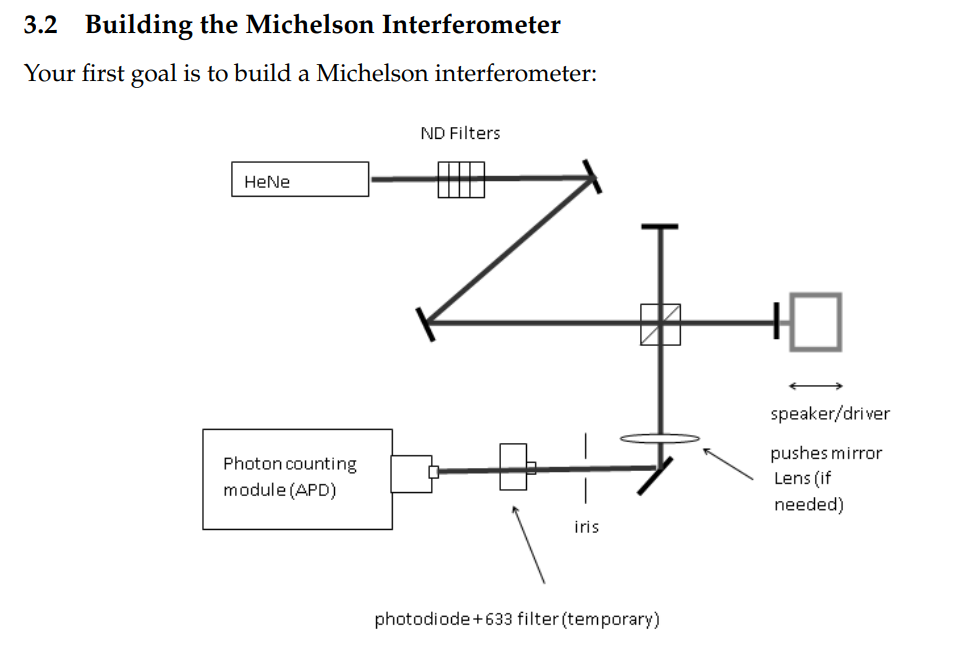
\includegraphics[width=0.8\textwidth]{physical.png} % Replace 'figure.jpg' with your image file
    \label{fig:setup}
\end{figure}

Our experimental apparatus is comprised of the laser, Michelson Interferometer, 
and the detector. Our HeNe laser has 65W power, and emits a red 
laser with a wavelength of $633nm$. The laser goes through 
the Michelson Interferometer, and the entangled ray is reflected 
to the detector. 

We install a ND filter between the beam splitter of the interferometer 
and the laser to reduce the number of photons that engage in 
the interference. Also, an iris is installed in order to extract 
the laser intensity of a specific point in the interference pattern. 
In order to minimize the detection of black room photons i.e. the extraneous 
photons that exist within the dark room, we install a 
633nm filter. The filter guarantees that the photons that hit the detector 
are solely from the HeNe laser. 

\begin{figure}[h]
    \centering
    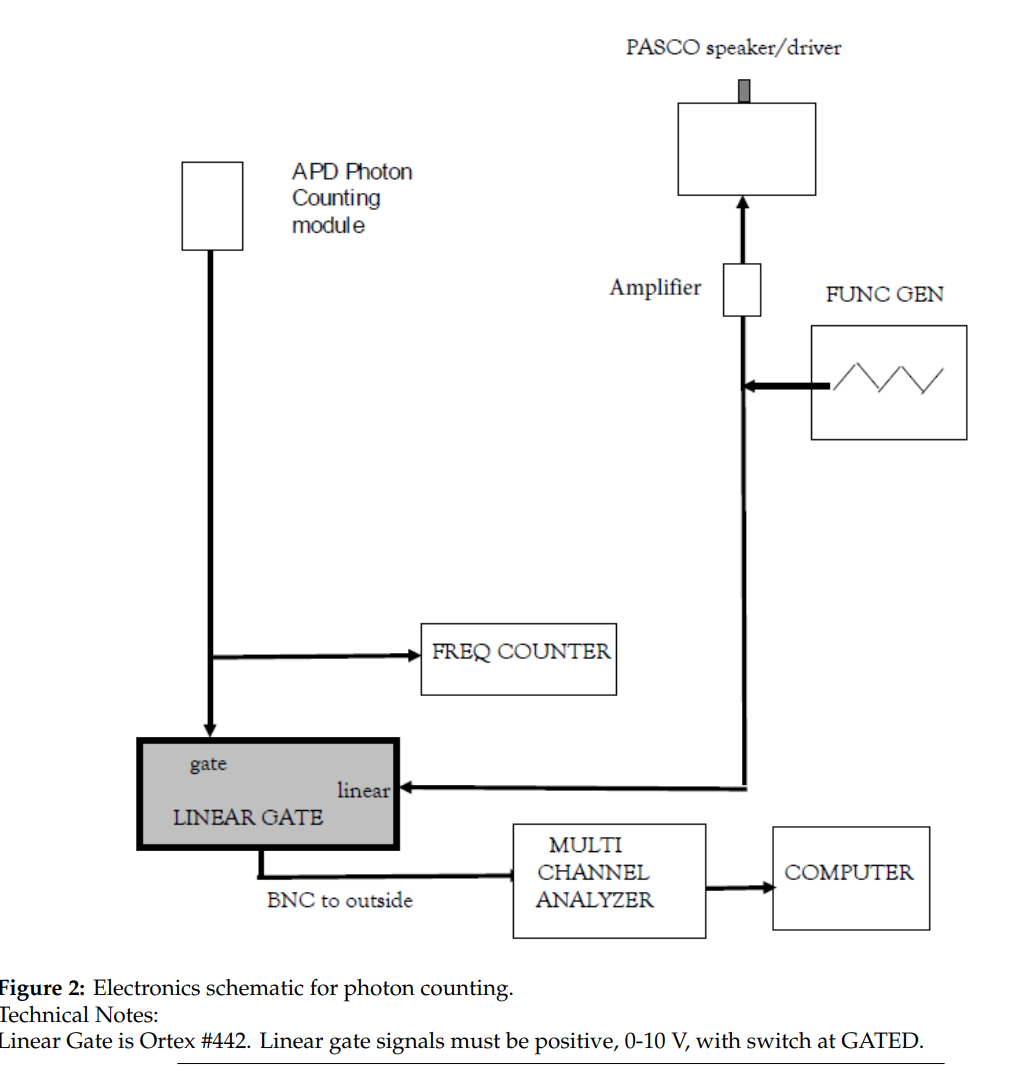
\includegraphics[width=0.8\textwidth]{electronics.png} % Replace 'figure.jpg' with your image file
    \label{fig:electronics}
\end{figure}

One leg of the Michaelson Interferometer oscillates according to the 
voltage from the function generator.
The voltage from the function generator is linked to the driver located 
at one end of the leg, leading the length of one end of the interferometer 
to change according to the function generator. 
By setting the function generator 
to send over triangular waves, we allow measurements of the 
photons to be made uniformly over the space. 

\begin{figure}[h]
    \centering
    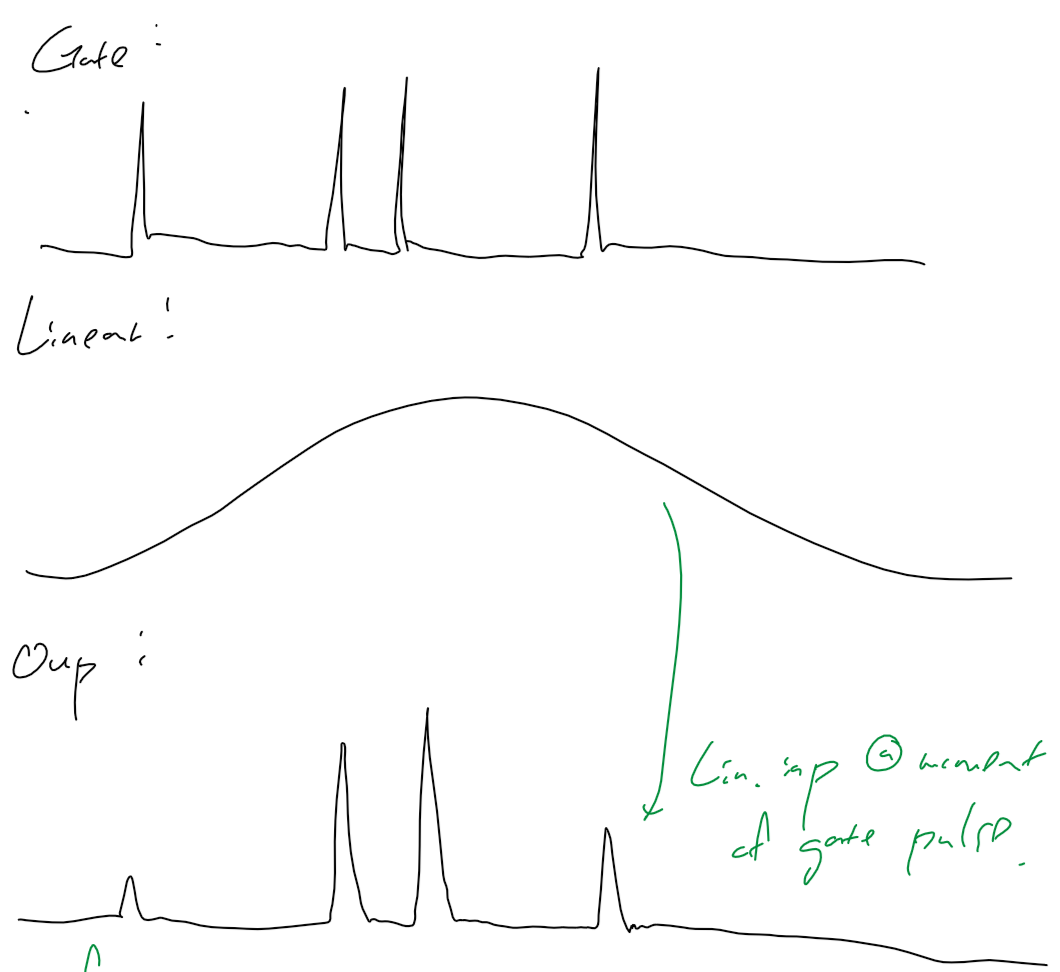
\includegraphics[width=0.8\textwidth]{lineargate.png} % Replace 'figure.jpg' with your image file
    \caption{Output of the Linear Gate}
    \label{fig:lineargate}
\end{figure}


From the NIM bin\footnote{NIM stands for Nuclear Instrumentation Module. 
It is a set of electronics built in the 1950's for nuclear and high energy physics. }, 
we will use the Linear Gate. The Linear gate takes input 
from two terminals, the "Linear" terminal and "Gate" terminal. Whenever 
a pulse is detected from the "Gate" terminal, the linear gate 
outputs a pulse that has the magnitude of the Linear terminal. 

By connecting the function generator to the "Linear" terminal and 
the photon detector to the "Gate" terminal, we can deduce the 
position of a certain photon. Our APD module gathers this data, and 
transmits to the MCA chanel analyser, which creates a historgram 
of photon counts for each voltage. 

Contrast is represented as intensity of light, and is the outcome between the difference between light bright and dark fringes. Contrast diminishes as light intensity goes down and can be seen when comparing ND10(higher intensity) to ND16(lower intensity).As fewer photons are able to interfere, the signal-to-noise ratio goes down, making the fringes less distinct. The sample data shows that although at ND 15 we can still see some contrast at ND16, the interference pattern becomes harder to detect and is likely due to the dark counts. 

Contrast decreases as light intensity drops and can be seen by looking at higher ND filters. At ND15 and ND16, both low intensity, the contrast is lower than what can be seen with ND10 and ND11 filters.
At ND 16, the photon count is so low that interference fringes are almost indistinguishable from background noise.
By considering the contrast formula:
\[
C \ = \  (I_{\rm max}-I_{\rm min})/I_{\rm max}+I_{\rm min}
\]
We can see that the lower the value of $I_{\rm max}$, due to less detectable photons, the bigger the impact of dark counts. 

%include Diagram

\section{Experimental Data}
%data from GPT
Due to a small accident, our alignment was disabled 
after the measurement of ND10. Thus, we have supplemented 
our data from the previous measurements made by
Professor Doret. The plotting of Professor Doret's data was done 
by a MATLAB script, written by ChatGPT. 



\begin{figure}[h]
    \centering
    \begin{subfigure}[b]{0.45\textwidth}
        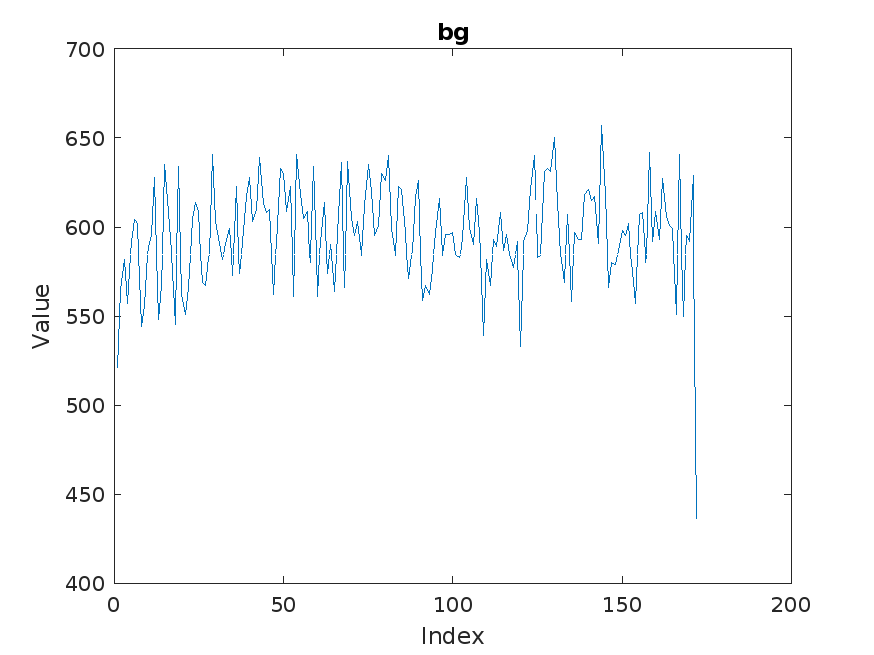
\includegraphics[width=\textwidth]{bg.png}
    \end{subfigure}
    \hfill
    \begin{subfigure}[b]{0.45\textwidth}
        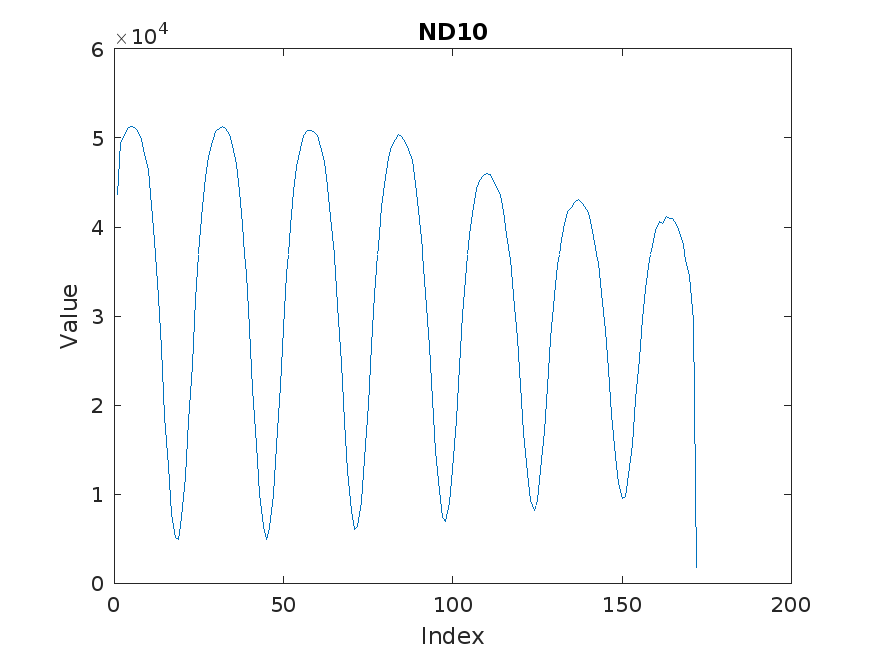
\includegraphics[width=\textwidth]{ND10.png}
    \end{subfigure}
    \
    \begin{subfigure}[b]{0.45\textwidth}
        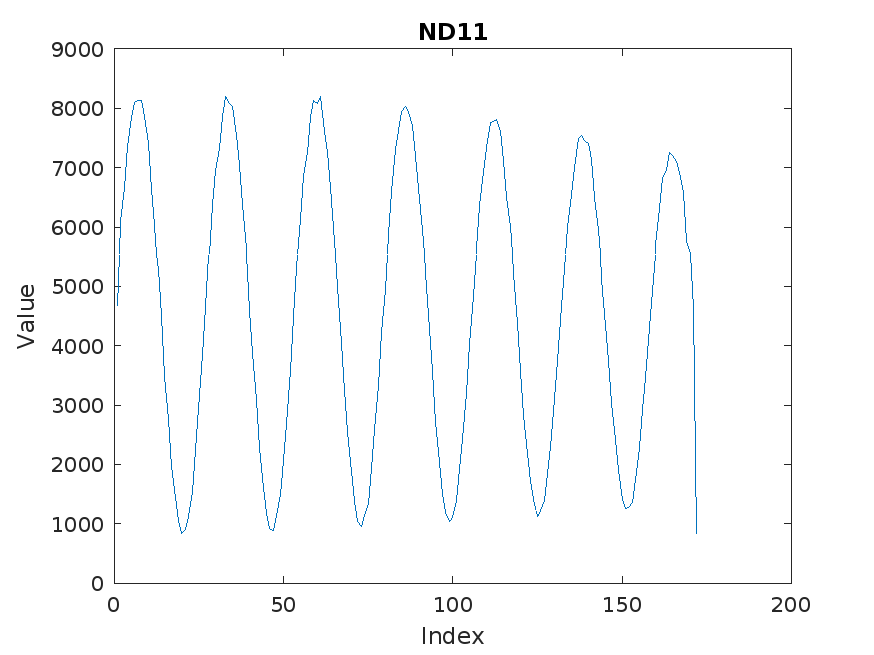
\includegraphics[width=\textwidth]{ND11.png}
    \end{subfigure}
    \hfill
    \begin{subfigure}[b]{0.45\textwidth}
        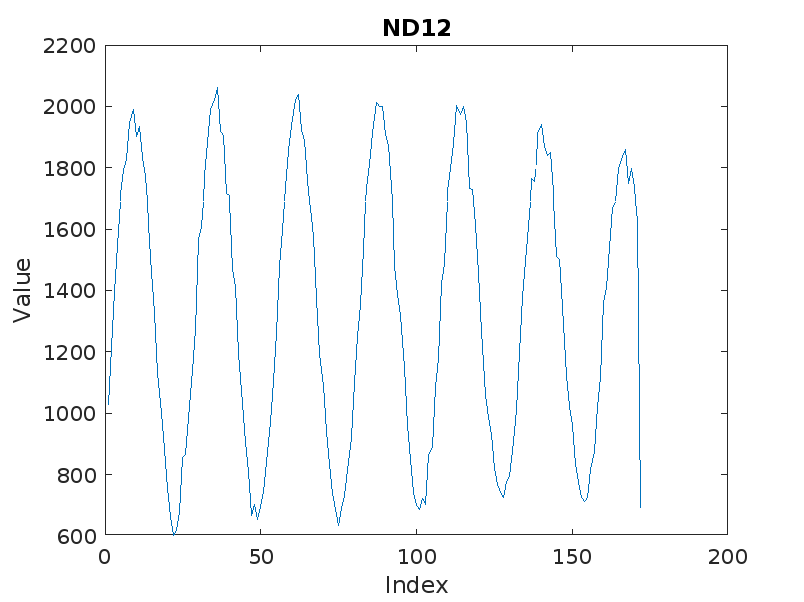
\includegraphics[width=\textwidth]{ND12.png}
    \end{subfigure}
    \caption{Raw Data: bg, ND10-ND12}
    \label{fig:bg-ND12}
\end{figure}


\begin{figure}[h]
    \centering
    \begin{subfigure}[b]{0.45\textwidth}
        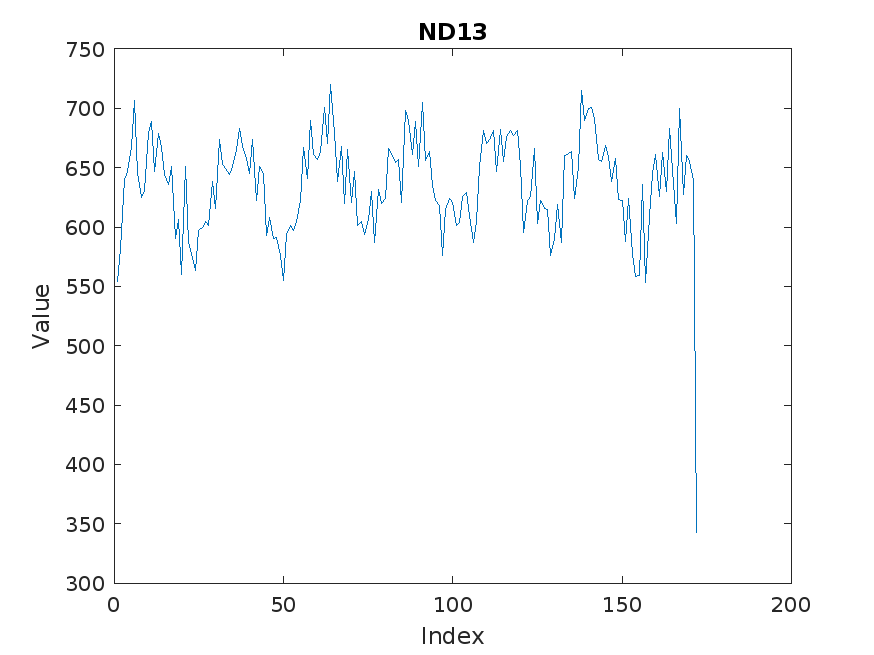
\includegraphics[width=\textwidth]{ND13.png}
    \end{subfigure}
    \hfill
    \begin{subfigure}[b]{0.45\textwidth}
        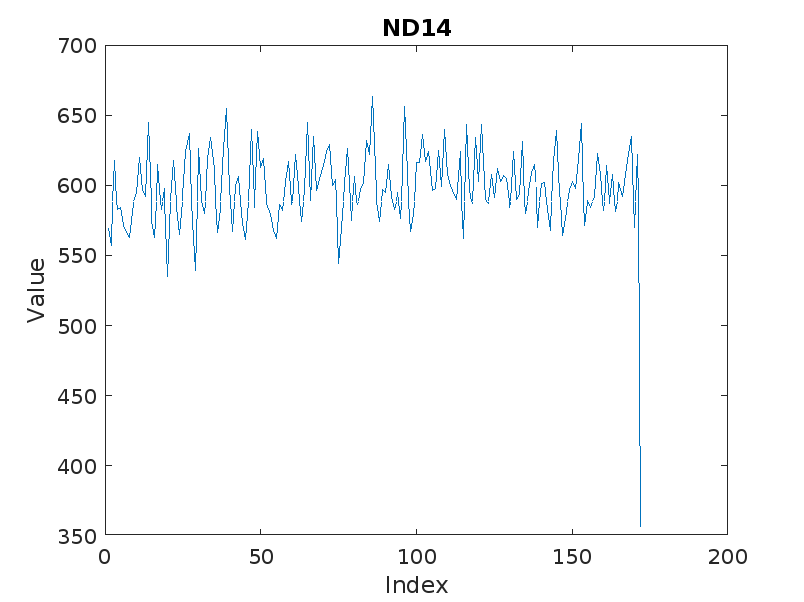
\includegraphics[width=\textwidth]{ND14.png}
    \end{subfigure}
    \
    \begin{subfigure}[b]{0.45\textwidth}
        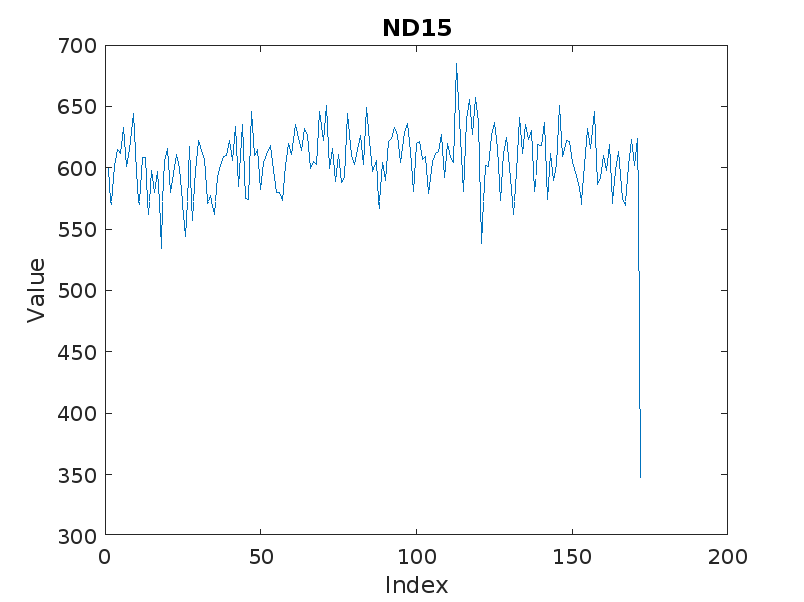
\includegraphics[width=\textwidth]{ND15.png}
    \end{subfigure}
    \hfill
    \begin{subfigure}[b]{0.45\textwidth}
        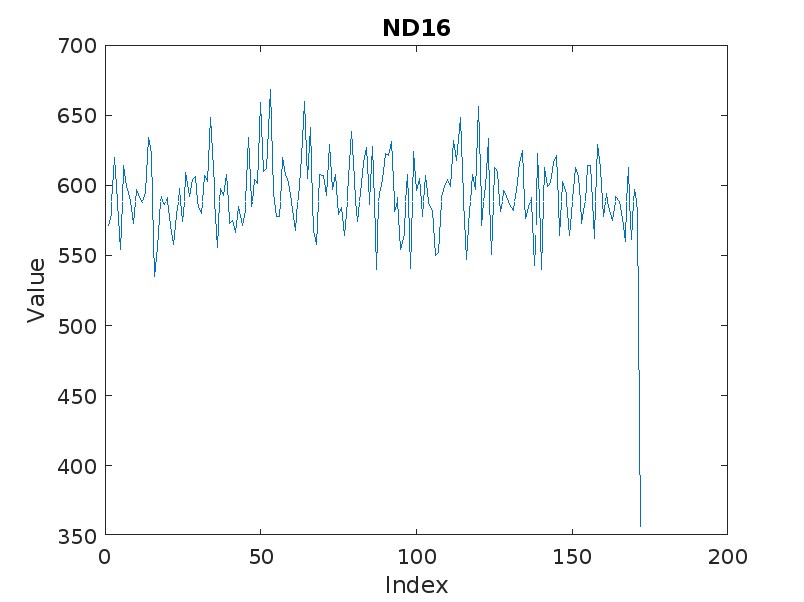
\includegraphics[width=\textwidth]{ND16.png}
    \end{subfigure}
    \caption{Raw Data: ND13-ND16}
    \label{fig:ND13-ND16}
\end{figure}


We also present the data with normalization and 
a sinusioid fit. The parameters $A, B, C, D$ specify the 
curve 
\begin{align}
    A\sin(Bx + C) + D
\end{align}

\begin{figure}[h]
    \centering
    \begin{subfigure}[b]{0.45\textwidth}
        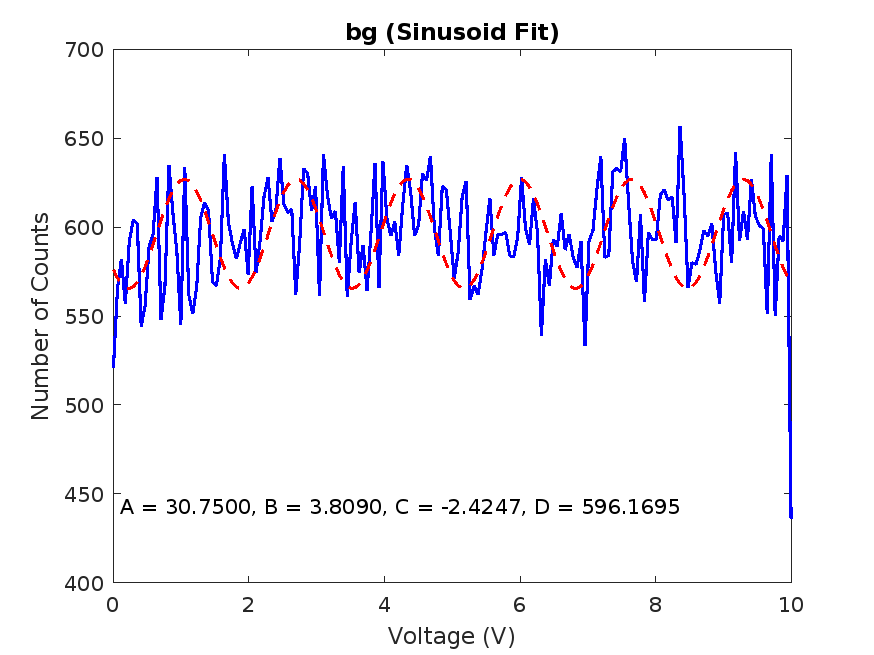
\includegraphics[width=\textwidth]{bg_sinusoid_fit.png}
    \end{subfigure}
    \hfill
    \begin{subfigure}[b]{0.45\textwidth}
        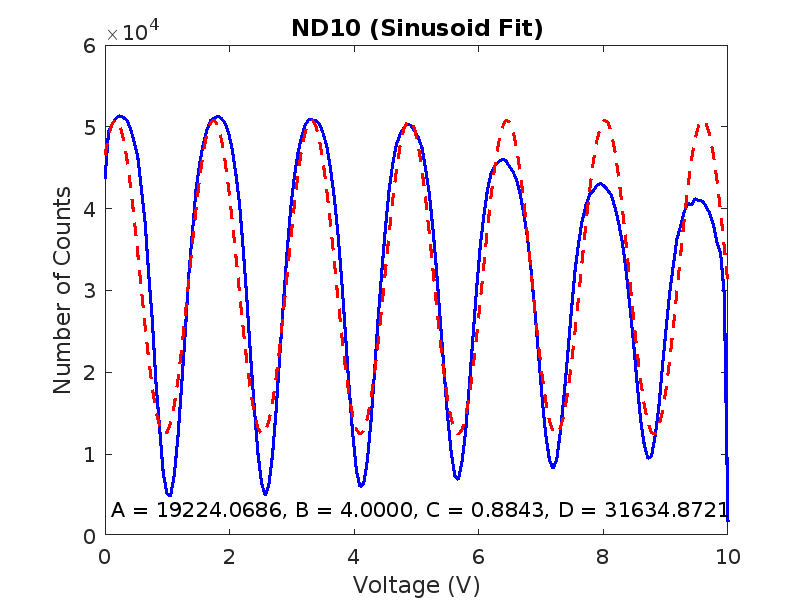
\includegraphics[width=\textwidth]{ND10_sinusoid_fit.png}
    \end{subfigure}
    \
    \begin{subfigure}[b]{0.45\textwidth}
        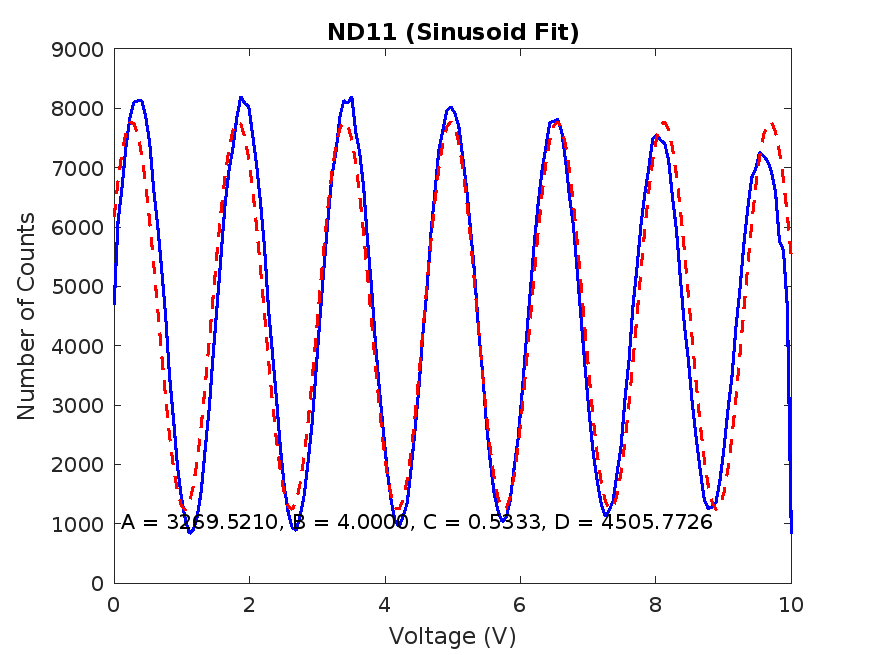
\includegraphics[width=\textwidth]{ND11_sinusoid_fit.png}
    \end{subfigure}
    \hfill
    \begin{subfigure}[b]{0.45\textwidth}
        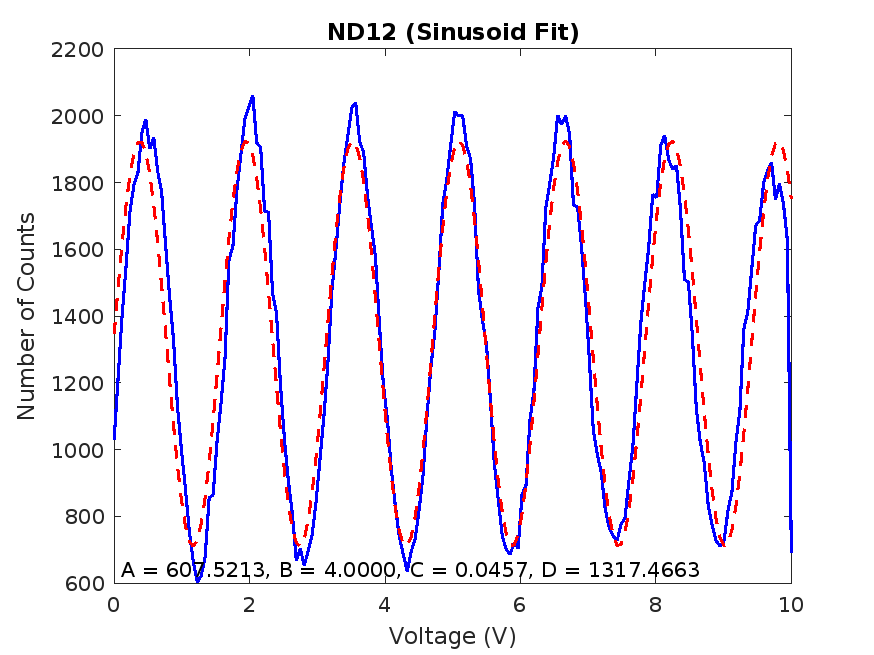
\includegraphics[width=\textwidth]{ND12_sinusoid_fit.png}
    \end{subfigure}
    \caption{Sinusoid Fit: bg, ND10-ND12}
    \label{fig:bg-ND12}
\end{figure}


\begin{figure}[h]
    \centering
    \begin{subfigure}[b]{0.45\textwidth}
        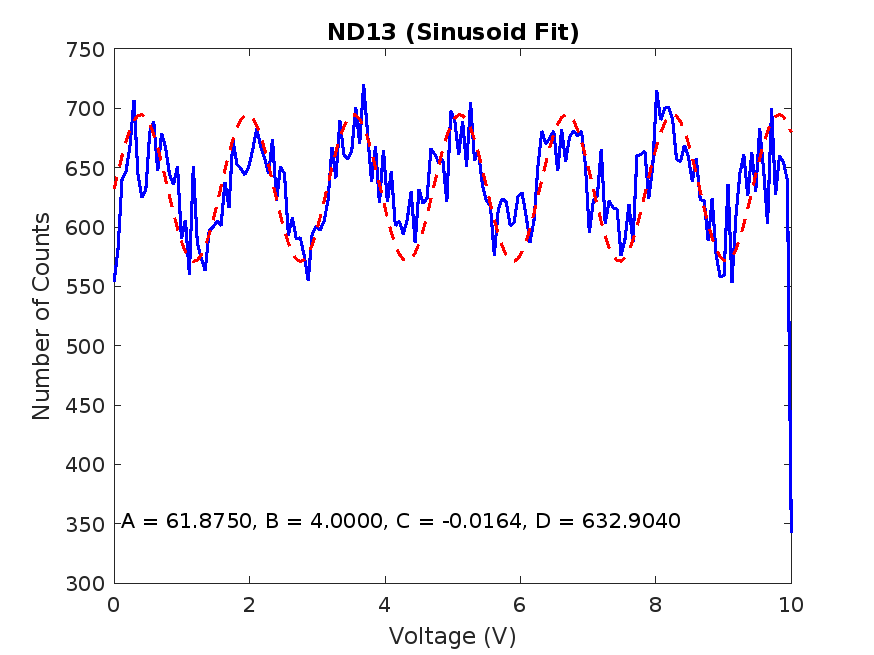
\includegraphics[width=\textwidth]{ND13_sinusoid_fit.png}
    \end{subfigure}
    \hfill
    \begin{subfigure}[b]{0.45\textwidth}
        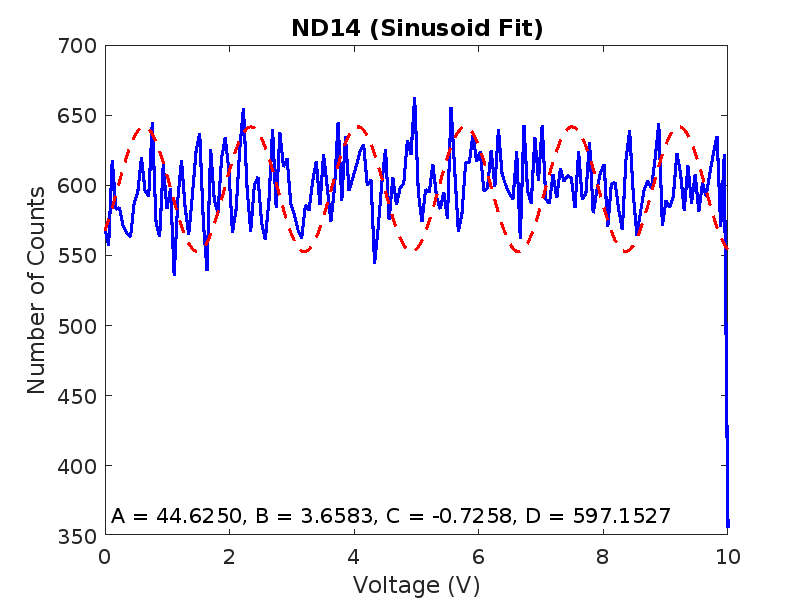
\includegraphics[width=\textwidth]{ND14_sinusoid_fit.png}
    \end{subfigure}
    \
    \begin{subfigure}[b]{0.45\textwidth}
        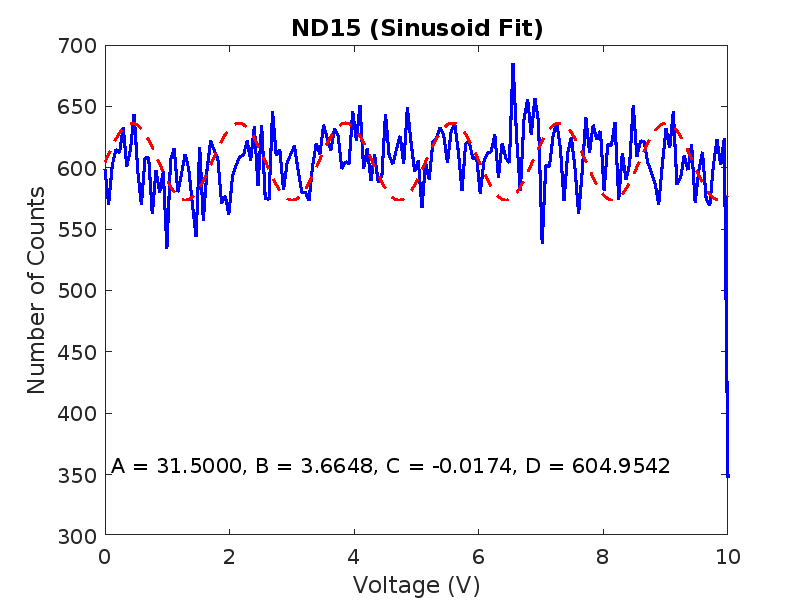
\includegraphics[width=\textwidth]{ND15_sinusoid_fit.png}
    \end{subfigure}
    \hfill
    \begin{subfigure}[b]{0.45\textwidth}
        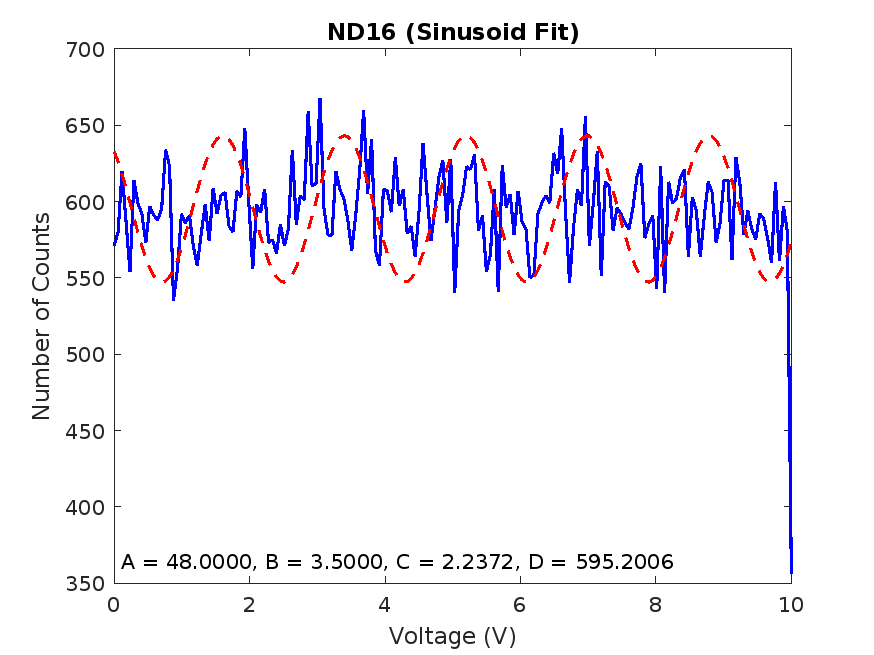
\includegraphics[width=\textwidth]{ND16_sinusoid_fit.png}
    \end{subfigure}
    \caption{Sinusoid Fit: ND13-ND16}
    \label{fig:ND13-ND16}
\end{figure}


\section{Analysis}

\textbf{Filter necessary to observe single photon interference}

In order to find out the domain in which the single 
photon interference happens, we first compute 
the necessary ND filter that allows the passage of a 
single photon per detection time. 

The energy of a single photon is governed by the wavelength. 
We know that the HeNe laser has a wavelength of 633nm. 
\begin{align}
    E_{ph} \ = \ \frac{h c} {\lambda} \ \approx \ 2.98 \cdot 10^{-19}
\end{align}


The sigle photon detector can make measurements up to the 
frequency of $f_{d} = 10^5 Hz$. Thus, if a single photon arrives at 
the detector for every time period $\tau \ = \ 1/f_d$, then 
the power received from the detector must be  
\begin{align}
    P_d \ = \ E_{ph} f_d \ = \ 2.98 \cdot 10^{-14} W
\end{align}

Applying the ND 15 filter allows an appropriate power output up to a magnitude. 
\begin{align}
    P_{\rm ND15} \ =\ P_{\rm HeNe} \cdot 10^{-15} \ = \ 65W \cdot 10^{-15} \ = \ 6.5 \cdot 10^{-14} W 
\end{align}
So if we observe a sinusoidial distribution in our data for the ND15 or 
ND16 measurement, we have verified the wave nature of a single photon. 

Using the $\chi$-squared test, we verify that the fit for ND15, ND16 is 
indeed proper. According to a MATLAB computation, the $\chi$-square value for 
the fit is 171 for both ND15, ND16. Given the degree of freedom of our 
fit is 168, we conclude that we have a good fit, and that we have 
observed single photon interference. 

\begin{figure}[htp]
    \centering
    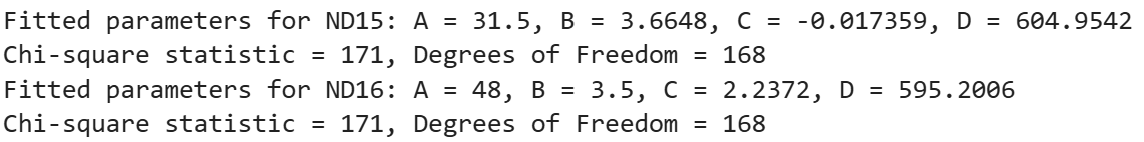
\includegraphics[width=0.8\textwidth]{ChiSq.png} % Replace 'figure.jpg' with your image file
    \caption{$\chi$-squared test results}
\end{figure}


%contrast v light level
%expected difference 

\section{Error and Uncertainty}

The photons follow a sub-poissonian statistic\footnote{
    In fact, it is also possible to verify the quantum model 
    by using sub-poissonian statistics of the photon count. 
    Instead of measuring the spacial distribution of the 
    photons, measure the time-dependent distribution. According to 
    the classical model, since the number of photons are always positive, 
    the variance of the count must be greater than the mean. Nonetheless, 
    in the quantum model, we can deduce that the variance can be less 
    than the mean by the Common Commutator Relations of the anhilitors. 
    So if the time-dependent distribution of the photon counts follow 
    a sub-poissonian distribution, then the quantum model is verified. 
}, assuming the quantum model. 
Therefore, the uncertainty of our measurement is around the square root 
of the absolute measurement. For example, if our measured count 
at the voltage bin $4.95V~5V$ is 2500, then the uncertainty will be 
50. Therefore we denote the count as 2500(50). 

As for the measurements made in ND15 and ND16, the average count 
over all bins are around 600. Hence we assume an error of $\sqrt{600} \approx 24.5$. 
This about 2/3 of the amplitude of the fit value for ND15, and 1/2 of the amplitude 
of the fit value for ND16. Therefore, considering the uncertainty of the measurement, 
we deduce that our measuremnt is inconclusive, and we need more counts in order to 
pinpoint single photon interference. 

ND Filters are the main source of loss in the beam path, but additionally other losses can come from the beam splitter, mirrors, and the APD detector. The APD’s 70 \% efficiency could have also contributed to loss. 

\section{Photon Count Rate and Spatial Distance Calculations}

To calculate the spatial distance between photons in the interferometer, we use the photon count rate and the speed of light. The spatial distance between photons, $D$, is given by:

\[
D = \frac{c}{C_R}
\]

where $c$ is the speed of light ($3 \times 10^8$ m/s) and $C_R$ is the photon count rate. For a count rate of 800,000 photons/sec, the spatial distance between photons is:

\[
D = \frac{3 \times 10^8 \, \text{m/s}}{800,000 \, \text{photons/sec}} = 375 \, \text{m}
\]

Thus, the average spatial distance between photons is 375 meters.

\subsection{Comparison of APD Count Rate to Predicted Photon Flux}

We compare the total number of avalanche photodiode (APD) counts per second to the predicted number of photons based on the Neutral Density (ND) filters. The ND filters attenuate light by a factor proportional to $10^{-\text{ND}}$. The predicted photon flux, $N_{\text{photons}}$, can be calculated as:

\[
N_{\text{photons}} = \frac{P}{E_p}
\]

where $P$ is the laser power (10 mW) and $E_p$ is the energy per photon ($3.14 \times 10^{-19}$ J). Substituting these values:

\[
N_{\text{photons}} = \frac{10 \times 10^{-3} \, \text{W}}{3.14 \times 10^{-19} \, \text{J}} = 3.18 \times 10^{16} \, \text{photons/sec}
\]

Thus, the source emits approximately $3.18 \times 10^{16}$ photons per second.

For a measured photon count rate of 800,000 photons/sec with an ND8 filter, we calculate the attenuation factor:

\[
A = \frac{N_{\text{initial}}}{N_{\text{final}}} = \frac{3.18 \times 10^{16} \, \text{photons/sec}}{800,000 \, \text{photons/sec}} = 3.18 \times 10^{11}
\]

\subsection{Accounting for APD Efficiency}

The APD detector's efficiency is 70\%, so the actual photon count rate is:

\[
C_{\text{actual}} = \frac{C_{\text{measured}}}{\eta}
\]

where $C_{\text{measured}}$ is the measured count rate and $\eta = 0.70$. Substituting the values:

\[
C_{\text{actual}} = \frac{800,000}{0.70} = 1,142,857 \, \text{photons/sec}
\]

\subsection{Error Propagation}

To account for uncertainties in the measured count rate and the detector efficiency, we calculate the relative uncertainty in the actual count rate using the formula:

\[
\frac{\Delta C_{\text{actual}}}{C_{\text{actual}}} = \frac{\Delta C_{\text{measured}}}{C_{\text{measured}}} + \frac{\Delta \eta}{\eta}
\]

The statistical uncertainty in the measured photon count rate is:

\[
\Delta C_{\text{measured}} = \sqrt{C_{\text{measured}}} = \sqrt{800,000} = 894.43
\]

The relative uncertainty in the measured count rate is:

\[
\frac{\Delta C_{\text{measured}}}{C_{\text{measured}}} = \frac{894.43}{800,000} = 0.00112 \, \text{or} \, 0.112\%
\]

The relative uncertainty in the detector efficiency is:

\[
\frac{\Delta \eta}{\eta} = \frac{0.01}{0.70} = 0.0143 \, \text{or} \, 1.43\%
\]

Thus, the total relative uncertainty in the actual count rate is:

\[
\frac{\Delta C_{\text{actual}}}{C_{\text{actual}}} = 0.00112 + 0.0143 = 0.01542
\]

The total uncertainty in the actual count rate is:

\[
\Delta C_{\text{actual}} = 0.01542 \times 1,142,857 = 17,616 \, \text{photons/sec}
\]

Thus, the final photon count rate, accounting for uncertainty, is:

\[
C_{\text{actual}} = 1,142,857 \pm 17,616 \, \text{photons/sec}
\]

\subsection{Analysis}

The APD detector’s efficiency significantly affects the photon count rate measurements. Since the detector is only 70\% efficient, the actual photon count rate is higher than the measured rate. The combined uncertainties from photon counting statistics and detector efficiency increase the overall error in the photon count rate. This effect becomes more pronounced at higher ND levels, where the photon count is lower and the impact of background noise and detector efficiency uncertainty is greater.


\section{Conclusion}
The objective of this experiment was to observe single-photon interference using a HeNe laser, Neutral Density (ND) filters, an ultra-sensitive avalanche photodiode (APD) detector, and a multi-channel analyzer to collect and analyze the resulting interference patterns. Although we were unable to use our own collected data, the provided sample data clearly demonstrated how increasing the attenuation (by adding ND filters) affected the interference pattern. As the light intensity decreased, especially at higher ND levels like ND15 and ND16, the contrast of the interference fringes became less distinct. This is expected, as higher attenuation leads to lower photon counts, making it more difficult to distinguish actual photon signals from background noise.
Despite the lower photon count at ND16, we were still able to fit a sinusoidal curve to the data, confirming the presence of an interference pattern. This outcome supports the quantum mechanical prediction that even at low intensities, photons can interfere with themselves, demonstrating wave-particle duality. The experiment ultimately reinforced the concept that even with fewer photons, the quantum nature of light persists, allowing us to observe interference, albeit with reduced clarity at higher ND levels.



\end{document}